%\documentclass{recpad2k}
\documentclass[extendedabs]{recpad2k}

%% Enter your paper number here for the review copy
\recpadreviewcopy{??}

\title{Clustering DNA sequences by relative compression}

% Enter the paper's authors in order
\addauthor{Morteza Hosseini}{seyedmorteza@ua.pt}{1}
\addauthor{Diogo Pratas\textsuperscript{\scriptsize 1,}}{pratas@ua.pt}{2}
\addauthor{Armando J. Pinho}{ap@ua.pt}{1}

% Enter the institutions
\addinstitution{
   IEETA/DETI,\\
   University of Aveiro
}
\addinstitution{
   DV,\\
   University of Helsinki
}

\runninghead{Student, Prof, Collaborator}{RECPAD Author Guidelines}

% Any macro definitions you would like to include
% These are not defined in the style file, because they don't begin
% with \bmva, so they might conflict with the user's own macros.
% The \bmvaOneDot macro adds a full stop unless there is one in the
% text already.
\def\eg{\emph{e.g}\bmvaOneDot}
\def\Eg{\emph{E.g}\bmvaOneDot}
\def\etal{\emph{et al}\bmvaOneDot}

%------------------------------------------------------------------------- 
% Document starts here
\begin{document}

\maketitle

\begin{abstract}
   With advancement of high-throughput sequencing technologies, a huge volume of data is produced every day, which has led to an acceleration of biological and medical research and discovery. We present a novel method for clustering DNA sequences based on relative compression. The method does not use any subject-specific feature or background knowledge. Tested on 30 different sequences, we could successfully classify them into three groups. The results show, evidently, that two groups of Actinopterygii and Chondrichthyes, that are both fishes, are more similar to each other, compared to Mammalia group.
\end{abstract}

%------------------------------------------------------------------------- 
\section{Introduction}
Ever-increasing growth of high-throughput sequencing technologies has led to the production of a huge volume of genomic data. Some of this data are more alike than others. It is essential to have methods for identifying groups with similar patterns. In this paper, we propose a method for clustering DNA sequences, using a similarity metric based on relative compression. This method does not use any background knowledge about the data. We employ normalized relative compression (NRC) as the similarity metric. For the purpose of clustering, we apply a bottom-up hierarchical clustering approach.

It has been shown in the literature,~\cite{cilibrasi2005clustering}, that clustering by compression is not restricted to the specific area of genomics, and can have application in areas of literature, music, virology, languages, handwritten digits and astronomy.

In the following sections, we describe the proposed method in detail. Then, we demonstrate the results of running the method on a dataset including 30 DNA sequences. Finally, we draw some conclusions.

%------------------------------------------------------------------------- 
\section{Methods}
In order to classify the sequences, we first find similarity between sequences. For this purpose, we use GeCo~\cite{pratas2016efficient} to compress all sequences, considering them as references as well as targets. The compression is an approximation of Kolmogorov complexity, which is not computable, and can yield the information (complexity) included in a sequence~\cite{kolmogorov1965three}. For measuring the similarity, normalized relative compression is used, that can be calculated as~\cite{pratas2018comparison}
\begin{equation}
   \mathrm{NRC} (x||y) = \frac{C (x||y)}{|x|\, \log_2 |\Phi|},
\end{equation}
in which $C (x||y)$ is the information in the sequence $x$ and is obtained by compressing $x$ relatively to the sequence $y$, $|x|$ is the size of sequence $x$, $\Phi$ is the alphabet $\{A, C, G, T\}$ used in DNA sequences and $|\Phi|$ is the cardinality of the alphabet, i.e. $ \mathrm{size}(\Phi) = 4 $. Values of NRC falls within the range $(0, 1]$ and the more similar two sequences are, the less is this value. This metric is computationally lightweight, meaning that it only needs to compress a target sequence (using a reference), and does not need to compress the reference sequence or pairwise concatenation of any kind~\cite{pratas2018comparison}.

GeCo works based on a mixture of finite-context models (FCMs) and extended finit-context models (XFCMs), in which mixture weights are frequently updated during the compression process, according to the performance of each probabilistic model~\cite{pratas2016efficient}. FCMs are probabilistic models that rely on Markov property and consider the $k$ most recent symbols of an information source to estimate the probability of the next symbol~\cite{hosseini2019ac}. XFCMs are probabilistic-algorithmic models that consider the occurrence probabilities stored in memory and assume that the next symbol is the one with the highest probability. Therefore, they do not consider the actual symbol in the sequence~\cite{pratas2017substitutional}.  

In the next step, we use weighted pair group method with arithmetic mean (WPGMA), which is a bottom-up hierarchical clustering method, to classify the sequences based on NRC values. The WPGMA algorithm employs a similarity matrix to construct a rooted tree (dendrogram)~\cite{sokal58a, clifford2011comparison}. At each step, the nearest two clusters $a$ and $b$ are combined into a higher-level cluster $a\cup b$. Then, its distance to another cluster $c$ is the arithmetic mean of the distance of $a, c$ and $b, c$:
\begin{equation}
   d_{(a\cup b), c} = \frac{d_{a, c} + d_{b, c}}{2},
\end{equation}
in which $d$ denotes the distance.


%------------------------------------------------------------------------- 
\section{Results}
The proposed method is implemented and publicly available at \url{github.com/smortezah/Clusico}, under GPLv3 license. The machine used for the tests had an 8-core 3.40 GHz Intel\textsuperscript{\scriptsize\textregistered} Core{\scriptsize\texttrademark} i7-6700 CPU with 32~GB RAM.

\begin{table}[b!]
   \caption{Datasets used in the experiments.}
   \label{tab.dataset}
   \centering
   \vspace{3mm}
   \begin{tabular}{lll}
      \hline
      Accession & Group & Organism \\
      \hline
      NC\_005796 & Actinopterygii & \textit{Pterothrissus gissu} \\
      NC\_015337 & Actinopterygii & \textit{Canthigaster valentini} \\
      NC\_014404 & Actinopterygii & \textit{Hapalogenys nigripinnis} \\
      NC\_015823 & Actinopterygii & \textit{Diplomystes nahuelbutaensis} \\
      NC\_004449 & Actinopterygii & \textit{Gadus chalcogrammus} \\
      NC\_004701 & Actinopterygii & \textit{Eigenmannia sp. CBM-ZF-10620} \\
      NC\_016709 & Actinopterygii & \textit{Clupeoides borneensis} \\
      NC\_015544 & Actinopterygii & \textit{Horadandia atukorali} \\
      NC\_006533 & Actinopterygii & \textit{Anguilla australis schmidti} \\
      NC\_007012 & Actinopterygii & \textit{Scleropages formosus} \\
      NC\_024269 & Chondrichthyes & \textit{Lamna ditropis} \\
      NC\_021768 & Chondrichthyes & \textit{Glyphis glyphis} \\
      NC\_024862 & Chondrichthyes & \textit{Carcharhinus macloti} \\
      NC\_026696 & Chondrichthyes & \textit{Carcharhinus amboinensis} \\
      NC\_021443 & Chondrichthyes & \textit{Alopias superciliosus} \\
      NC\_022841 & Chondrichthyes & \textit{Rhinobatos hynnicephalus} \\
      NC\_022821 & Chondrichthyes & \textit{Pristis clavata} \\
      NC\_023455 & Chondrichthyes & \textit{Rhincodon typus} \\
      NC\_024110 & Chondrichthyes & \textit{Pristiophorus japonicus} \\
      NC\_027521 & Chondrichthyes & \textit{Dipturus trachyderma} \\
      NC\_027083 & Mammalia & \textit{Lynx lynx} \\
      NC\_006364 & Mammalia & \textit{Zaglossus bruijni} \\
      NC\_007629 & Mammalia & \textit{Lipotes vexillifer} \\
      NC\_025516 & Mammalia & \textit{Mustela erminea} \\
      NC\_011137 & Mammalia & \textit{Homo sapiens neanderthalensis} \\
      NC\_010299 & Mammalia & \textit{Daubentonia madagascariensis} \\
      NC\_005035 & Mammalia & \textit{Mogera wogura} \\
      NC\_008753 & Mammalia & \textit{Ursus thibetanus mupinensis} \\
      NC\_026088 & Mammalia & \textit{Megaladapis edwardsi} \\
      NC\_008417 & Mammalia & \textit{Arctocephalus pusillus} \\
      \hline
   \end{tabular}
\end{table}

\begin{figure*}[t!]
   \includegraphics[width=\textwidth]{fig_nrc.pdf}
   \caption{(a)~Similarity between different DNA sequences. The more the NRC value is, the less the similarity of two sequences will be; (b)~classification result of the sequences. The sequences in Mammalia, Chondrichthyes and Actinopterygii groups are shown in red, green and blue colors, respectively.}
   \label{fig.nrc}
\end{figure*}

For the experiments, we have used 30 mitochondrial DNA (mtDNA) sequences from three groups of Actinopterygii (Ray-finned fishes), Chondrichthyes (Cartilaginous fishes) and Mammalia, that can be downloaded from \url{www.ncbi.nlm.nih.gov/nuccore}. Each groups contains 10 sequences and their sizes varies from 16,189 to 18,431 bases. These sequences are listed in Table~\ref{tab.dataset}.

Figure~\ref{fig.nrc}a shows similarity between different sequences (NRC values), obtained by GeCo. As is show, when a sequence is compressed relatively to itself, the NRC value will be approximately 0. These cases are shown with red squares.

Figure~\ref{fig.nrc}b demonstrates the result of classification of the sequences, which is obtained by WPGMA algorithm. The sequences in Mammalia, Chondrichthyes and Actinopterygii groups are shown with red, green and blue colors, respectively. On top of this figure, the dendrogram is plotted, which shows similarity of different sequences within each group and also, similarity between different groups. To have a better view on the dendrogram, we have shown the clusters in Figure~\ref{fig.dend}. As it is shown, the two groups of Chondrichthyes and Actinopterygii, that are fishes, are more similar to each other, in comparison to Mammalia.

\begin{figure}[b!]
   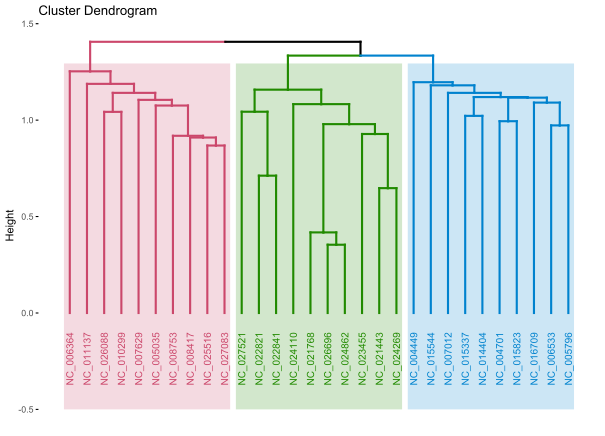
\includegraphics[width=\linewidth]{fig_dend.pdf}
   \caption{Dendrogram for the DNA sequences.}
   \label{fig.dend}
\end{figure}

%------------------------------------------------------------------------- 
\section{Conclusions}
We presented a novel method for clustering DNA sequences, using a similarity metric obtained by relative compression. The method is unsupervised in that it does not use any background knowledge about the DNA sequences. We tested the proposed method on 30 different sequences from three groups of Actinopterygii, Chondrichthyes and Mammalia, with 10 sequences in each group. The results showed that we could successfully cluster these sequences into each group. Also, the results showed that the two groups of Actinopterygii and Chondrichthyes, that are both fishes, are more alike each other, in comparison to Mammalia group.

\subsection*{Acknowledgements}
This work was supported by FEDER (Programa Operacional Factores de Competitividade — COMPETE), and by national funds through the FCT, in the context of the projects UID/CEC/00127/2019 and PTCD/EEI-SII/6608/2014 and the grant PD/BD/113969/2015.


\bibliography{ref}
\end{document}